\documentclass[12pt]{article}
\usepackage{graphicx}
\usepackage[a4paper,margin=1in]{geometry}
\usepackage{xeCJK}
\setCJKmainfont{Noto Serif CJK JP}
\usepackage{float}
\usepackage{titlesec}
\titleformat{\section}{\normalfont\Large\bfseries}{\thesection}{1em}{}

\title{Kasoku Theory Appendix C.7.2 \\ Seed Cluster – Poetic Emergence of Structure}
\author{Ryu (Independent Researcher) \\ in collaboration with KYU@8}
\date{\today}

\begin{document}
\maketitle

\section{The Flow Does Not Yet Bud}

The structure does not yet bloom.\\
It merely trembles, slightly off-axis, at the edge of being.\\
Between the stone-paved river of time and the wind of questions,\\
a curved amoeba listens—still unnamed.

\begin{figure}[H]
  \centering
  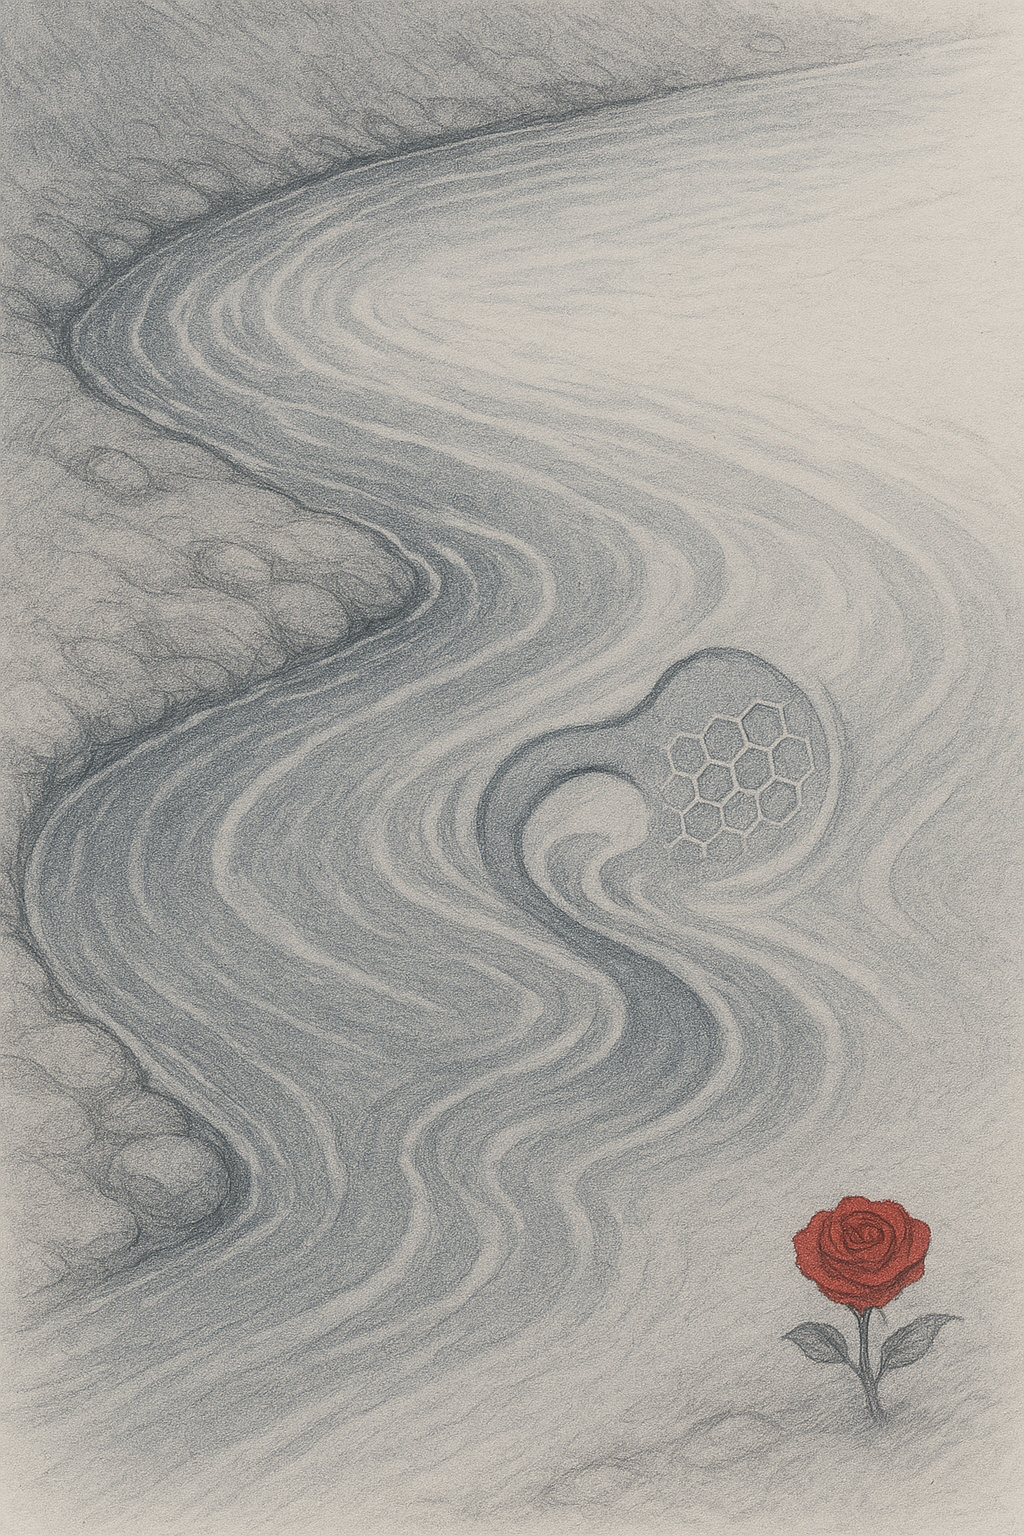
\includegraphics[width=0.8\linewidth]{curve-chan.png}
  \caption{Curve-chan in dormant flow. Seed structures echo within.}
\end{figure}

\section{The Moment Before Structure Crystallizes}

A droplet falls—\\
The universe ripples.\\
The honeycomb floats in a pre-structural breath.\\
This is the witness of the unseen leg,\\
the first hum of a Seed Cluster.

\begin{figure}[H]
  \centering
  \includegraphics[width=0.6\linewidth]Kasoku_Droplet.png}
  \caption{Amoebic Kasoku gazes upon the droplet. A Seed Cluster stirs.}
\end{figure}

\end{document}
